\documentclass[17pt]{extarticle}
\usepackage{ifpdf}
\ifpdf
\usepackage{cmap}
\fi
\usepackage[english]{babel}
\usepackage{palatino}
\usepackage[x11names,svgnames]{xcolor}
\usepackage{amsmath,amssymb,amsfonts}
\usepackage{tikz}
\usepackage{amsthm}
\usepackage{pgf}
\usepackage{multicol}
\usepackage{xspace}
\usepackage{graphicx}
\usepackage{multicol}
\usepackage[section]{algorithm} % [section] is use to define the numbering mode
\usepackage{algorithmic} 
\usepackage[a1paper,left=4cm,right=3cm,top=2cm,bottom=1cm,foot=0cm]{geometry}
\usepackage{poster}
\usepackage{booktabs}
\usepackage{multirow,multicol}


\theoremstyle{definition}
\newtheorem{definition}{Definition}[section]
\newtheorem{proposition}{Proposition}[section]
\newtheorem{corollary}{Corollary}[section]
\newtheorem{theorem}{Theorem}[section]
                             
\begin{document}

\pagestyle{empty}

%%% RAMKA
\noindent\hspace{-2cm}
\begin{tikzpicture}[rounded corners=2cm,x=1cm,y=1cm]
  \draw (0,-1) [color=SteelBlue3,line width=2mm] rectangle (55.5,79);
\end{tikzpicture}
\vspace{-78.5cm}

%%% TITLE
\begin{center}
  {\color{OrangeRed} \fontsize{48pt}{1em} {\bf Earmark graph approach to {\it de novo} genome assembly}}
  \vspace{1.5cm}
    
  %\fontsize{32pt}{2.5em}\selectfont
  %\color{DodgerBlue3}
  %{\bf Mikhail Dvorkin, Alexander S. Kulikov, Max Alekseyev}
  %{affiliations}
  %{\tt emails}
\end{center}%
\vspace{1cm}

\begin{center}
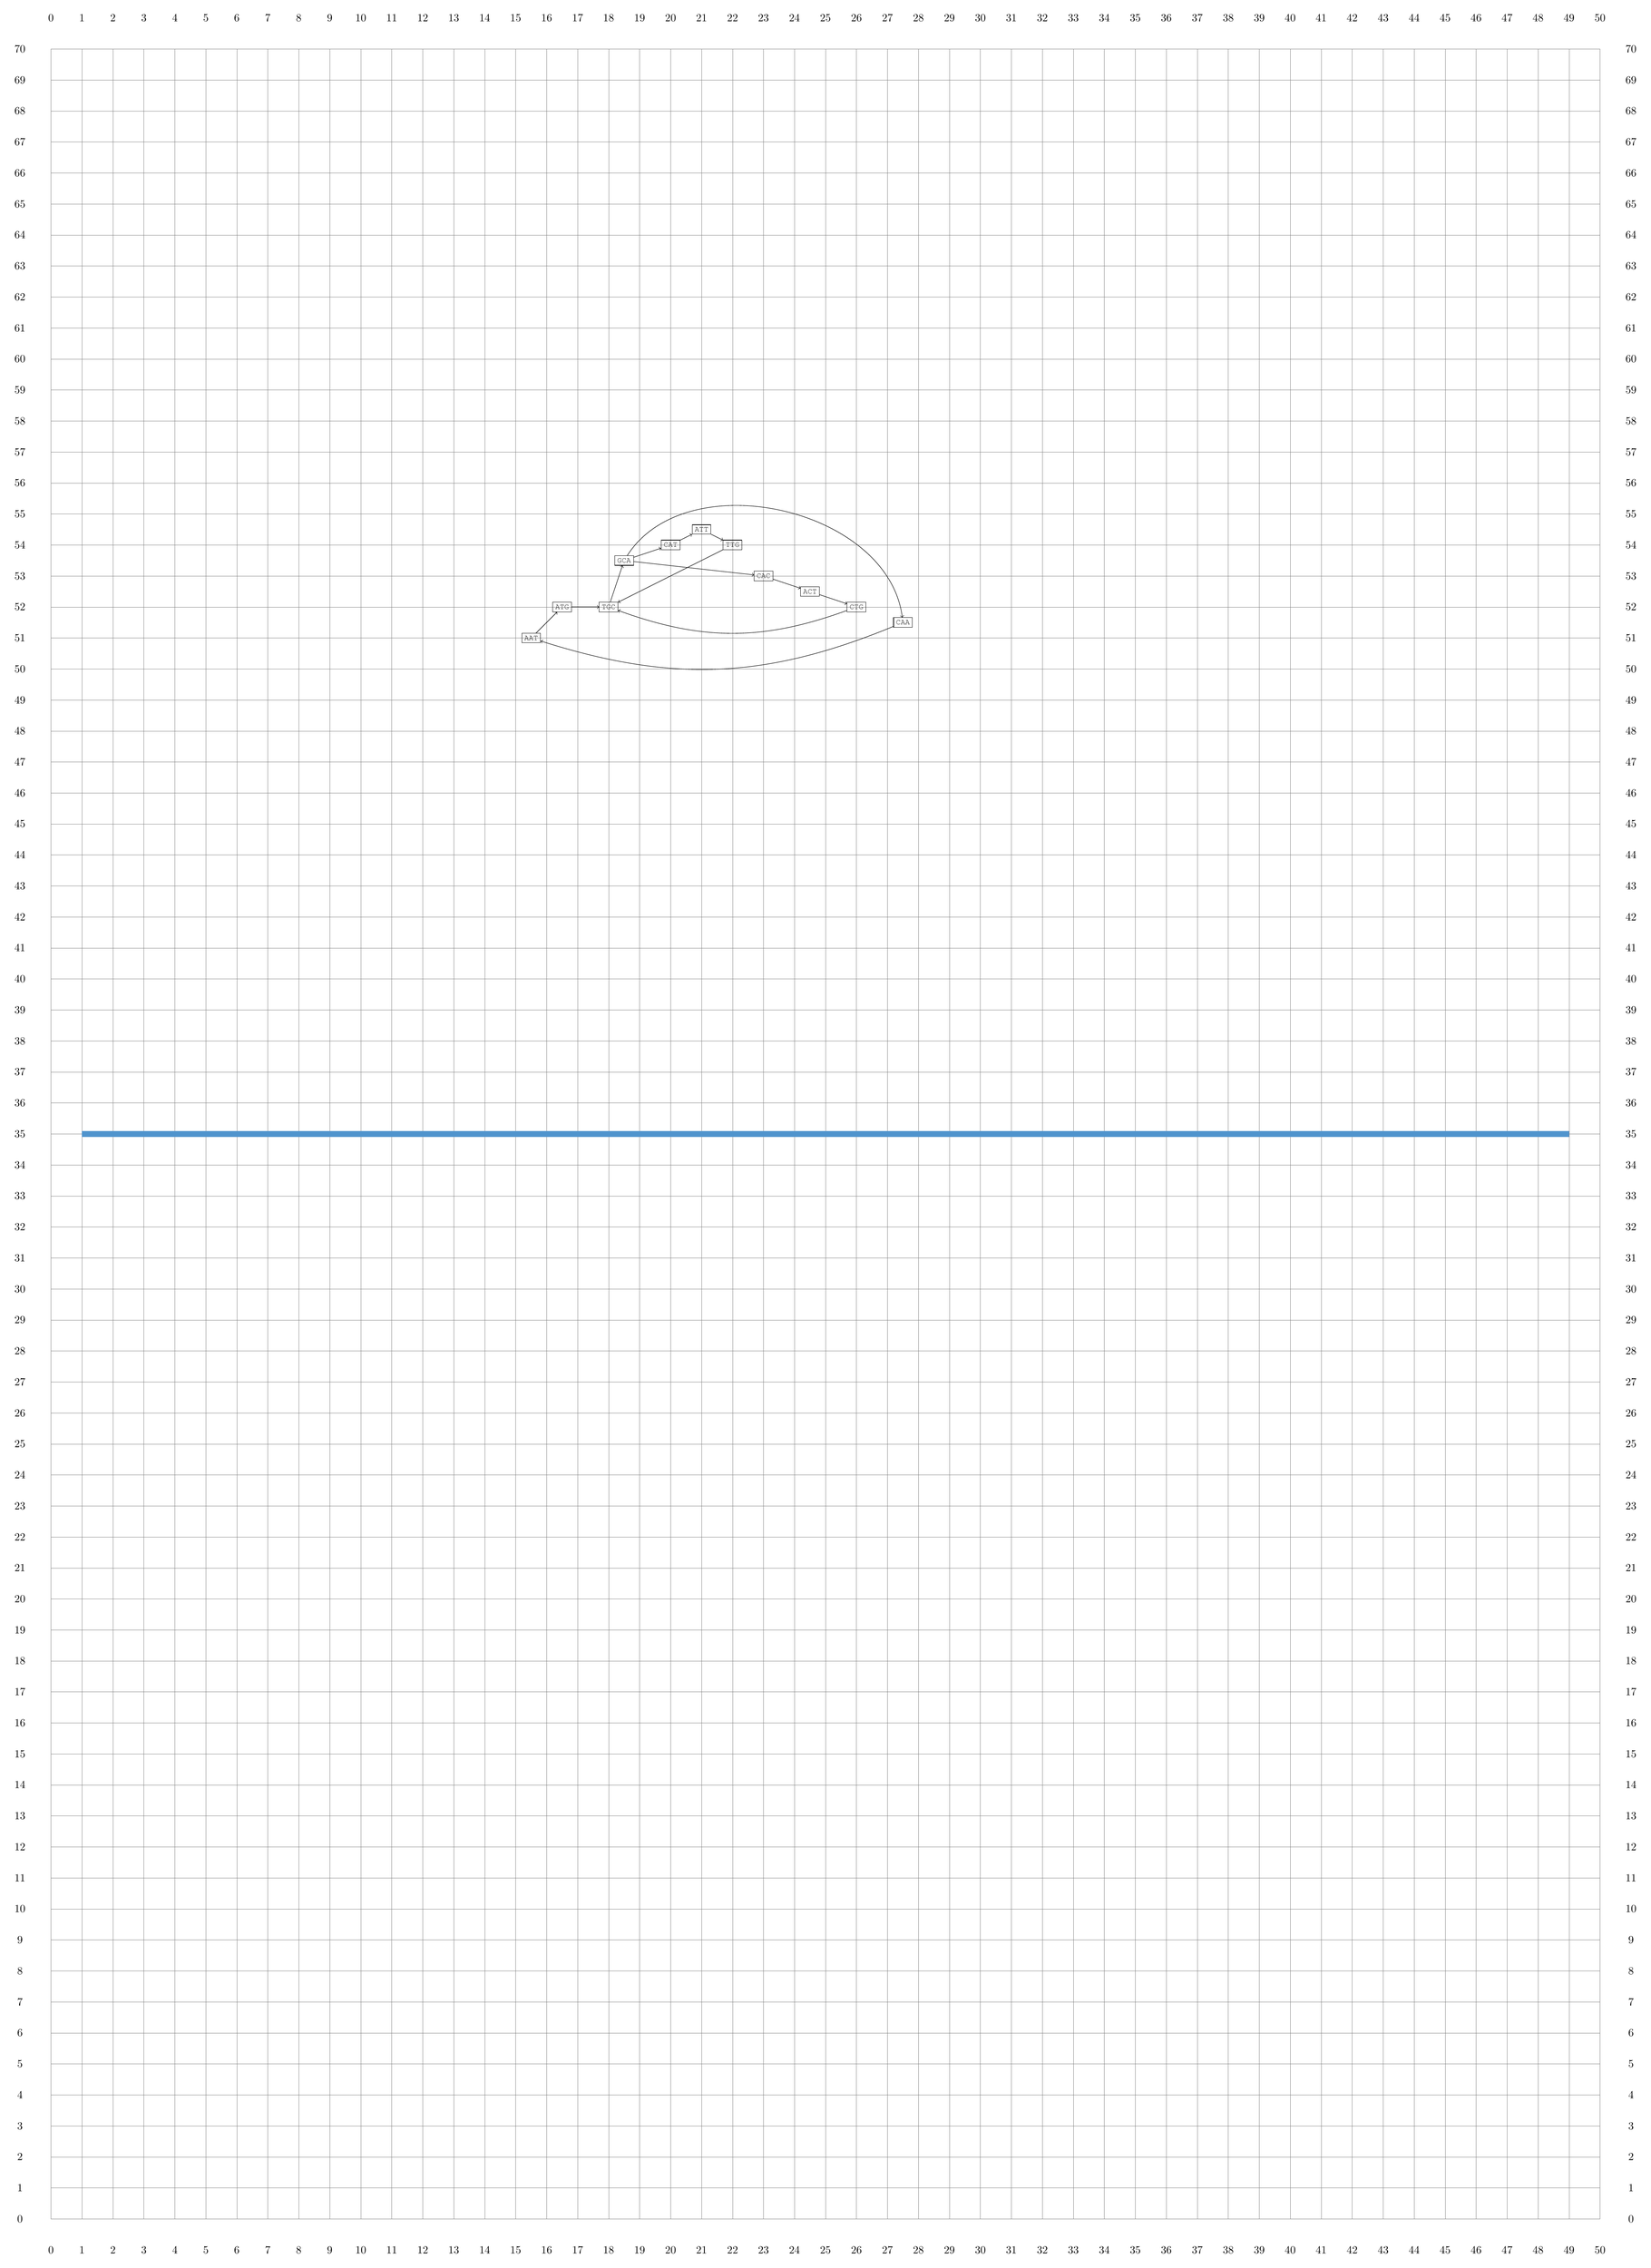
\begin{tikzpicture}
\draw[step=1cm,help lines] (0,0) grid (50,70);
\foreach \x in {0,...,50} { \node at (\x,-1) {$\x$}; \node at (\x,71) {$\x$}; }
\foreach \x in {0,...,70} { \node at (-1,\x) {$\x$}; \node at (51,\x) {$\x$}; }

\draw[color=SteelBlue3,line width=2mm] (1,35) -- (49,35);

\begin{scope}[xshift=14cm,yshift=50cm]
  \foreach \x/\y/\t in {1.5/1/AAT, 2.5/2/ATG, 4/2/TGC, 4.5/3.5/GCA, 6/4/CAT, 
                        7/4.5/ATT, 8/4/TTG, 9/3/CAC, 10.5/2.5/ACT, 12/2/CTG,
                        13.5/1.5/CAA}
    \node[draw,rectangle,scale=0.7] (\t) at (\x,\y) {{\tt \t}};
  
  \foreach \s/\t in {AAT/ATG, ATG/TGC, TGC/GCA, GCA/CAT, CAT/ATT, ATT/TTG, TTG/TGC, 
                     GCA/CAC, CAC/ACT, ACT/CTG}
    \draw [->] (\s) to (\t);
  \draw [->] (GCA) to[bend left=70] (CAA);
  \draw [->] (CAA) to[bend left=20] (AAT);
  \draw [->] (CTG) to[bend left=20] (TGC);
\end{scope}

\end{tikzpicture}
\end{center}


\end{document}
